%%
%% copyright quintard julien
%%
%% kaneton
%%
%% design.tex
%%
%% path          /home/mycure/kaneton/view/cursus/schedule
%%
%% made by mycure
%%         quintard julien   [quinta_j@epita.fr]
%%
%% started on    Fri Feb  4 15:10:05 2005   mycure
%% last update   Mon Oct 31 22:28:51 2005   mycure
%%

%%
%% --------- packages ---------------------------------------------------------
%%

\documentclass[10pt,a4wide]{article}
\usepackage[english]{babel}
\usepackage{a4wide}
\usepackage{graphicx}
\usepackage{fancyheadings}
\usepackage{multicol}
\usepackage{indentfirst}
\pagestyle{fancy}

\setlength{\footrulewidth}{0.3pt}
\setlength{\parindent}{0.3cm}
\setlength{\parskip}{2ex plus 0.5ex minus 0.2ex}

%%
%% --------- header -----------------------------------------------------------
%%

\lhead{\scriptsize{The kaneton distributed operating system}}
\rhead{\scriptsize{The kaneton scheduling}}
\rfoot{\scriptsize{EPITA Computer System Laboratory - www.lse.epita.fr}}

\title{The kaneton scheduling}

\author{\small{Julien Quintard} \\
        \scriptsize{EPITA Computer System Laboratory, Paris, France}}

\date{\scriptsize{\today}}

\begin{document}

\maketitle

%
% --------- text --------------------------------------------------------------
%

\begin{multicols}{2}



\textbf{kaneton} is a project of the EPITA specialisation year in system,
network and security.

The goal of the project is to give students a complete view of an operating
system.

The project is composed of two important parts: the \textbf{microkernel}
and the {distributed operating system}.

For the moment the distributed operating system is not developed by the
students.

Every group, composed of about four students, has to develop many parts
of the kaneton microkernel.

To do so, the professors give students a development environment containing
everything needed to start the project.

The whole project is divided into parts, each part must be validated by
the students.

The project comes with three courses:

\begin{itemize}
  \item
    \textbf{kaneton}: this course is intended to give students a good overview
    of operating system design problems and introduced the kaneton design.
  \item
    \textbf{kernel}: this course give a complete study of the kernel
    internals including microkernels, memory management, processes and threads,
    synchronisation, communications, and complete case studies.
  \item
    \textbf{Intel architecture}: this course will explain the Intel
    architecture including the instructions sets to the memory management
    and finally to the task management.
\end{itemize}

Let's see the year scheduling:

\begin{itemize}
  \item
    \textbf{k0}: the students will have to learn low-level programming to
    understand the processor programming interface and the different
    memory management modes. This part is called the bootstrap.
  \item
    \textbf{k1}: the students will develop a bootloader. Its role is to
    build an memory environment for the futur kernel execution. In this
    project, the students will learn to deal with a new memory model
    and to develop in a very strict environment, from scratch.
  \item
    \textbf{k2}: this project will lead the students to an higher abstraction
    level. The goal of the project is to develop parts of the set manager,
    the id manager, the address space manager and finally the segment
    manager to be able to manage physical memory.
  \item
    \textbf{k3}: this project introduces the development of some drivers
    and a the development of the region manager to provide virtual memory
    operations.
  \item
    \textbf{k4}: the students will have to develop the task manager, the
    thread manager and the scheduler to provide the kaneton microkernel
    the possibility to create execution contexts.
  \item
    \textbf{k5}: this project leads the students to the communications
    into the microkernel and to the development of some microkernel servers.
  \item
    \textbf{kn}: this project is a free one. Each group has to choose the
    subject of this project, to design, to implement and to document
    the project. The themes for this project are: distributed aspects and/or
    security ones.
\end{itemize}



\end{multicols}



\begin{figure}[h]
\centerline{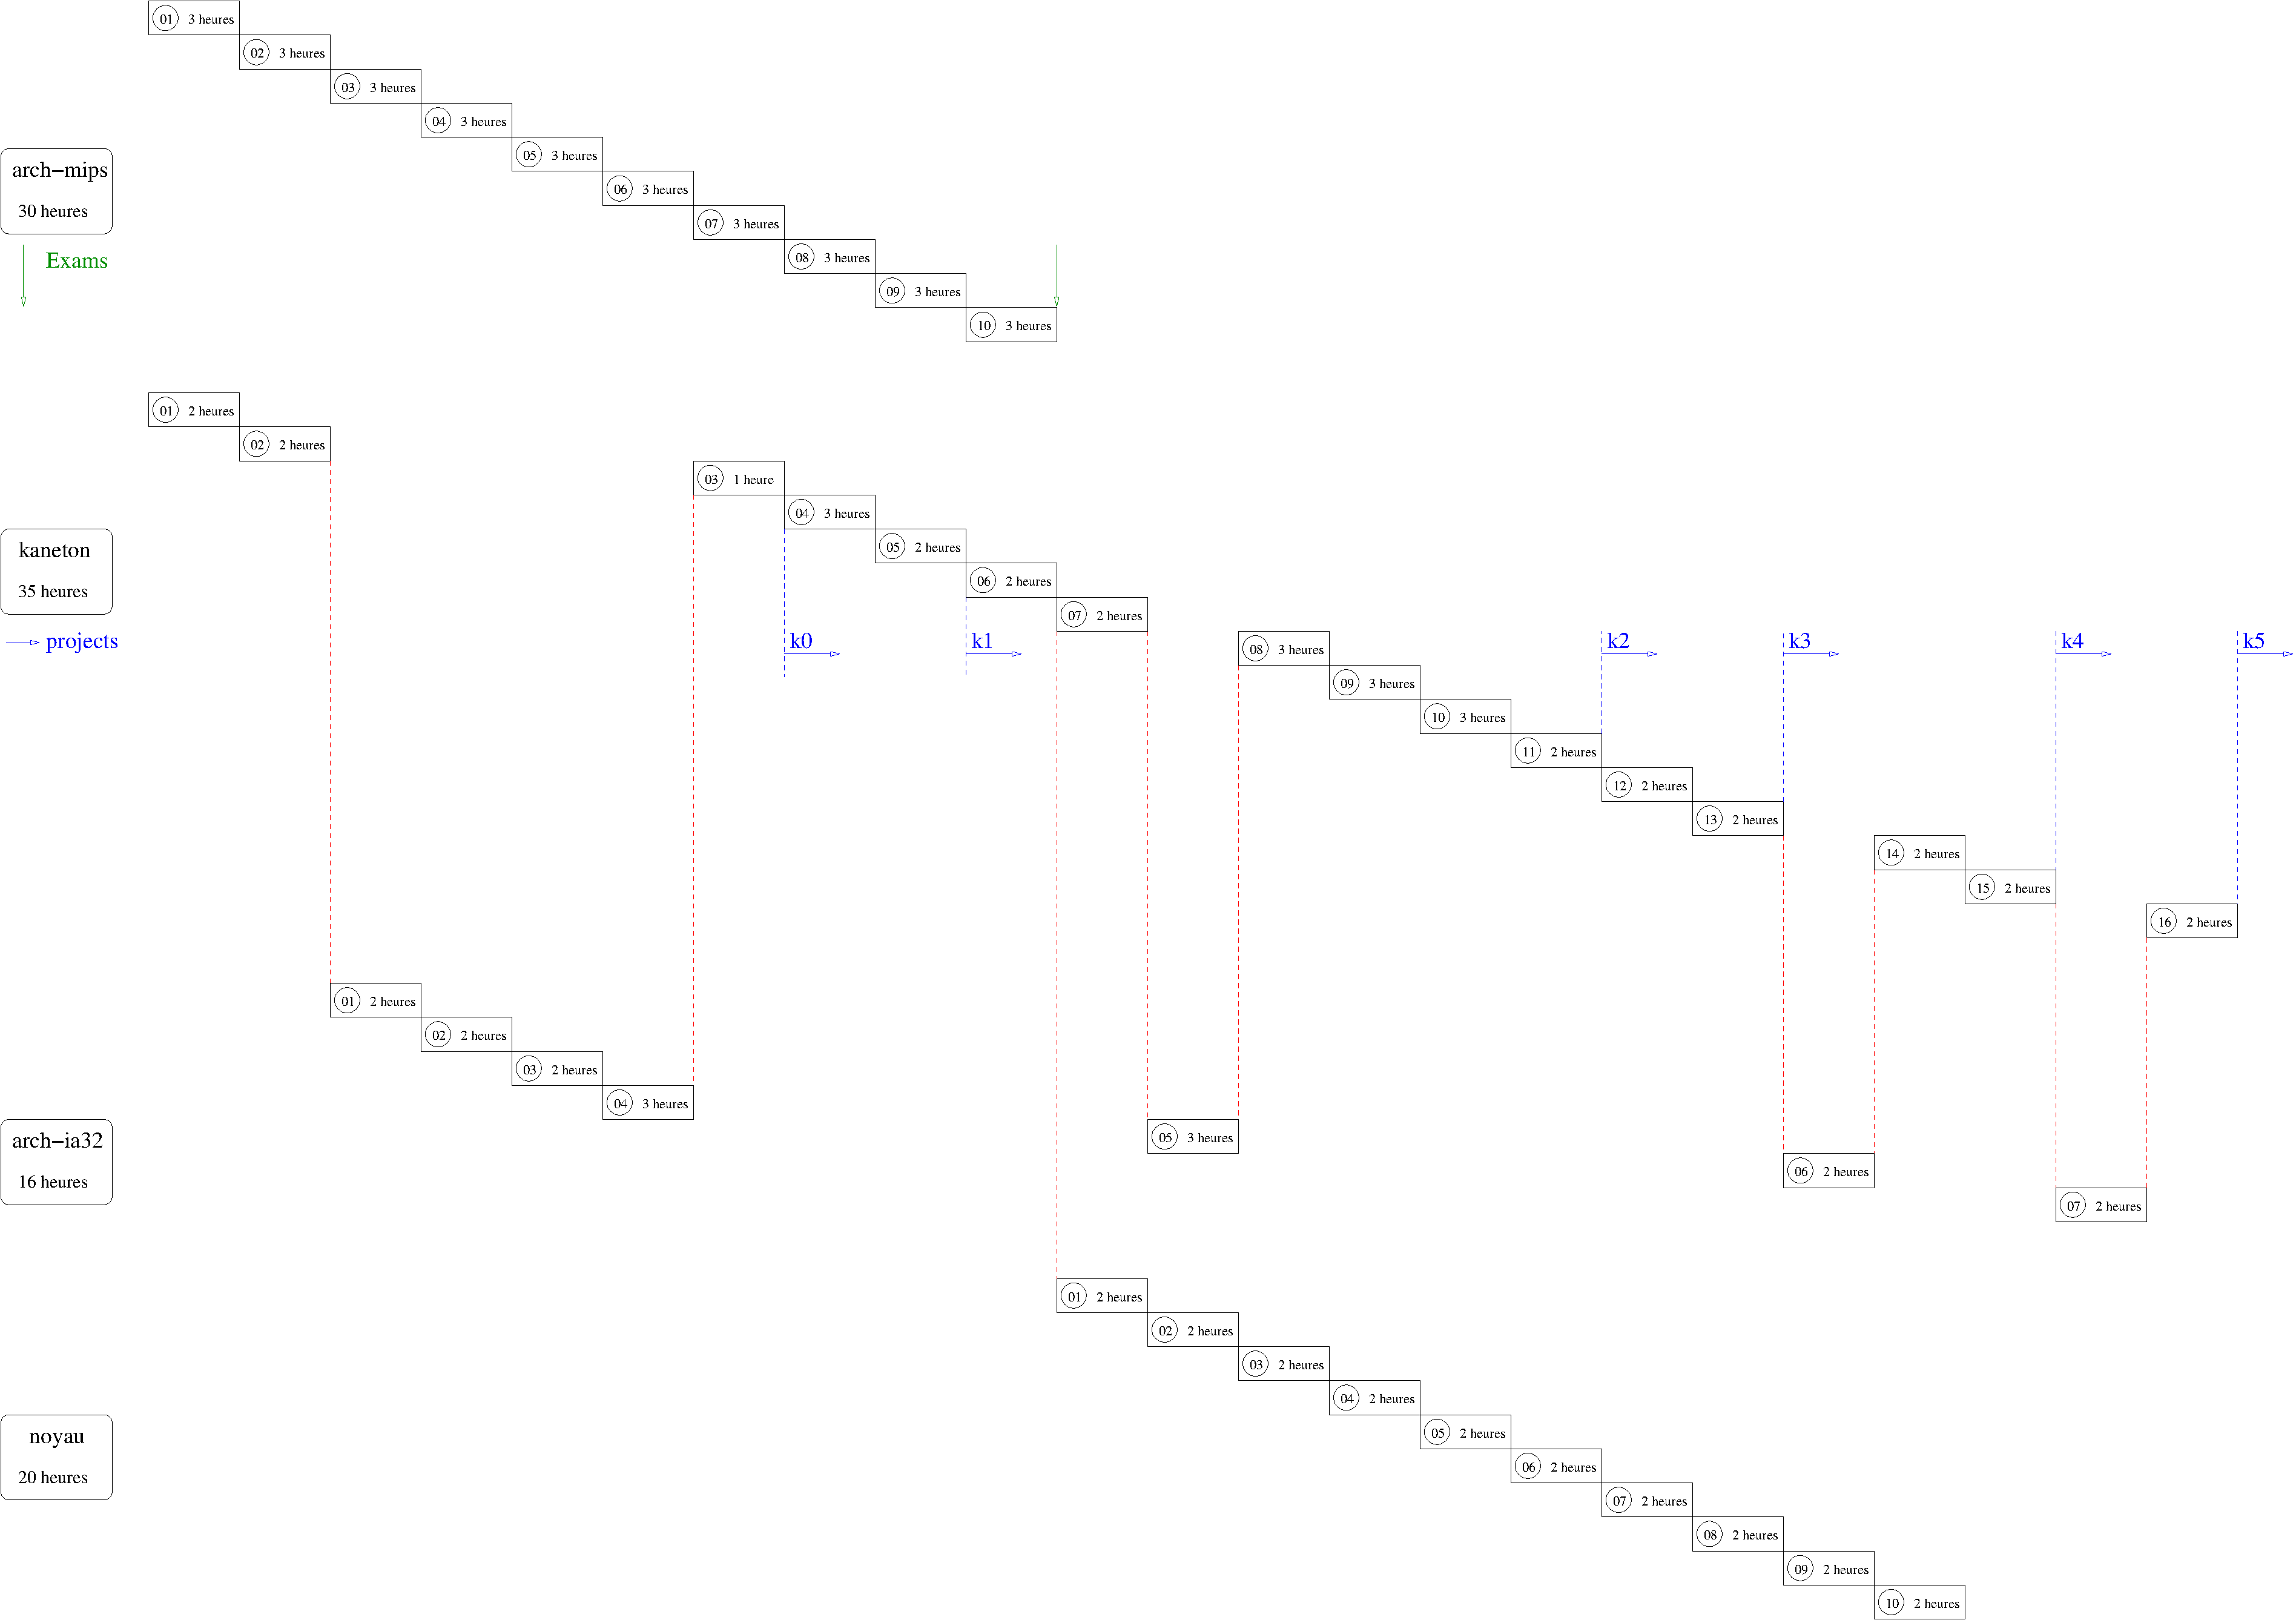
\includegraphics{figures/schedule.eps}}
\end{figure}



\end{document}
